\documentclass[../598comp.tex]{subfiles}

\graphicspath{ {./lectures/images/}{./images/} }

\date{05-21}

\begin{document}

\section{05-21}

\subsection{Existence of Unsolvable Problems}

Modern language makes this proof much easier than it was for Turing.
\begin{theorem}
  There is no algorithm that can analyze algorithms and their inputs and
  determine whether the algorithm halts or not on the given input.
  \begin{proof}
    Write $S$ for an algorithm. $S(x)$ for running algorithm on input $x$. $\#S$
    for the code of $S$. Everything used to have to be coded up as an integer.
    $S(w) \shortdownarrow$ indicates that $S$ halts when run on $w$. $S(w)
    \shortuparrow$ for when $S$ runs forever on the given input.

    Assume we have a program $H(\#S, x)$ that returns true if $S(x)
    \shortdownarrow$ and false if $S(x) \shortuparrow $. $H$ itself always halts.

    Define $P(x) \coloneqq$ if $H(x, x)$ then loop forever else halt.

    Now we give $P$ it's own code. The question is $P(\#P) \shortdownarrow$ or
    $P(\#P) \shortuparrow$. Two cases
    \begin{enumerate}
    \item 
      If $P(\#P) \shortdownarrow$, then $H$ returns true but this means that $P$
      loops. Contradiction
    \item
      If $P(\#P) \shortuparrow$, then $H$ returns false but this means that $P$
      halts. Contradiction
    \end{enumerate}
    Therefore a program like $P$ cannot exist. 
  \end{proof}
\end{theorem}

\subsection{Turing Machine}

\href{https://cs.mcgill.ca/~prakash/Courses/598/Notes/turing_machines.pdf}{Notes}

$\delta(q, a) = (q', b, L)$ means if the machine reads $a$ and is in state $q$,
it changes state to $q'$, writes $b$ in the place of $a$ and moves one step to
the \ul{left}.

At each stage only a finite amount of information is processed.

Easy to see that $\{a^nb^nc^n \mid n \geq 0\}$ can be recognized by a turning
machine.

A \ul{configuration} of a TM is a description of its state, the tape, and the
position of the reading head. Convention that you write all of the tape to the
left of the state, then the state, and then the rest of the tape including the
cell the head is looking at.

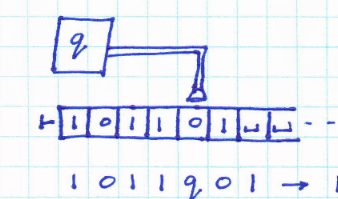
\includegraphics[width=\textwidth]{example_configuration}

With this you can move backwards in the ``stack'' without deleting information.

$uaq_ibv$ yields $uq_jacv$ if $\delta(q_i, b) = (q_j, c, L)$. Emphasis on how
only a three letter window is affected.

Acceptance of $w$ by $M$. Start in a start configuration $q_0w$. Follow the
transitions and end up in the accept state. Once you get to the accept state you
can't leave.

A new phonomenon: The machine may go into an infinite loop. This doesn't happen
in DFA or NFA because you read left to right and you are done.

The language of a machine. $L(M) = \{ w \mid M \ \text{halts and accepts} \ w\}$.

If $w \notin L(M)$ it does not mean that $M$ explicitly rejects $w$. It could be
looping forever. Basically there is a new ``I don't know'' option which makes a
huge difference. Not everything can be answered.

\begin{definition}[Turing Recognizable]
  $L$ is \ul{Turing Recognizable} if $\exists TM \ M$ such that $L = L(M)$.

  We say computably enumerable or CE for recognizable.
\end{definition}

\begin{definition}[Turing Decidable]
  $L$ is \ul{Turing Decidable} if $\exists TM \ M$ such that $\forall w, \ M(w)
  \shortdownarrow$ and $L = L(M)$. i.e. for every word you get a Yes/No answer.

  We say \ul{computable} for decidable.
\end{definition}

\begin{fact}
  Any decidable language is, of course recognizable.
\end{fact}

\begin{note}
  Old terminology. Recursively enumerable (RE) for CE. Recursive for decidable.
\end{note}

\subsection{Models of Computation}

One can think of a turing machine as a computing function $f: \NN \to \NN$
instead of accepting languages. They are equivalent, but sometimes it is more
helpful to think in one way than the other.

People proposed many variations all of which turned out to be equivalent to
turing machine. Examples include Multitape Turing Machine, Nondeterministic
Turing Machine, n-dim TM, Post Machine, 2 stack NFA, 2 counter, RAM using
assembler, while programs, any modern programming language, $\lambda$-calculus,
conbinatory logic, phrase structure grammas, post systems. This is not to
say that some are not differences in efficiency/ease.

Are \ul{all} possible formalisms equivalent? We don't know for sure but it is
believed so. Church-turing thesis says so.

So we believe there isa notion of computable functoin independent of any
specific model of computation.

Proved that certaint hings were impossible but in a completely different sense.
When referring to distributed computing, the notion of what is computible 

Turing machine writes down all the prime numbers. Never going to write them all
because there are infinitely many.

If you define computing to be looking at the answer one it halts, if you say you
have one TM who's tape is being fed into a second TM, the first guy doesn't even
have to halt before being useful.

\subsection{Theory of Computability}

We say 2 infinite sets are equipollent if $\exists$ a bijection between them.
There is no bijection between $\NN$ and $2^\NN$ but there is a bijection between
$\NN \times \NN \to \NN$.

\begin{definition}[Equipollent]
  Two sets are said to be equipollent if there is a bijective function mapping one onto the other.

  "Equipollent" means "of equal power", where "power" here alludes to the size of the sets. Two sets are equipollent precisely if they have the same cardinality.
\end{definition}

We now have algorithms that may loop forever and produce no output. We model
this by \ul{partial functions}, $f: \NN \to \NN$. Partial means that $f$ is not
defined for every $n \in \NN$. Let $f(n) \shortdownarrow$ mean $f$ is defined on
$n$ and $f(n) \shortuparrow$ mean $f$ is not defined on $n$.
\begin{gather*}
  dom(f) = \{n \mid f(n)\shortdownarrow\}
\end{gather*}
$f = g$ as partial functions means $dom(f) = dom(g)$ and $\forall n \in dom(f),
f(n) = g(n)$. New notion that we don't typically have is $f \leq g$ means that
$dom(f) \subseteq dom(g), \ \forall n \in dom(f), \ f(n) = g(n)$. This gives a
partial order structure.

There is a \ul{minimal element}, i.e. the everywher undefined function. It's
domain is the empty set.

\begin{gather*}
  range(f) = \{m \mid \exists n \in dom(f) \ \text{s.t.} \ f(n) = m\}
\end{gather*}

When discussing computability, $\NN$ is not important; no real difference
between $\NN$, $\NN^k$, and $\Sigma^*$. $\RR$ is not comparable because
uncountable; there is a fascinating field concerning $\RR$ but we won't discuss
it here.

\begin{note}
  It is not algorithmic to write things like:
  \begin{enumerate}
  \item 
    wait for $M$ to halt, if it doesn't halt then...
  \item
    Check on \ul{every} word if...
  \end{enumerate}
\end{note}

\begin{definition}[Computable Function]
  A function $f: \NN \to \NN$ is computable if there is an algorithm $A$ such
  that for all $n \in dom(f)$, $A$ halts and the output if $f(n)$.
\end{definition}

\begin{definition}[Computable/Decidable Set]
  A set of natural numbers $X \subseteq \NN$ is \ul{computable} or \ul{decidable}
  if its characteristic function
  \begin{gather*}
    \chi_x(n) =
    \begin{cases}
      1, &n \in X \\
      0, &n \notin X
    \end{cases}
  \end{gather*}
  it \ul{total computable}.
\end{definition}

\begin{definition}[Total function]
  A \ul{total function} is defined for all possible input values.
\end{definition}

\begin{proposition}
  An infinite set of natural numbers is \ul{decidable} iff it is the range of a
  total non decreasing computable function.
  \begin{proof}
    Suppose we have $X$, we have $f$ as above $X = range(f)$ and we have an
    always terminating algorithm for $f$ called $A$. Let $x$, want to know if $x
    \in X$.

    Run $A$ on $0, 1, 2, 3, \dots$. Eventually you may get $A(n) = x$ then say
    yes $x \in X$. Or you may get $A(n) > x$ then stop and say no, $x \notin X$.

    For the reverse direction, assume we have a decision procedure for $X$, call
    it $B$. Run $B$ on $0, 1, 2, \dots$. As soon as it says ``Yes'' for the the
    first time you say $f(0) = x_0$. Second time you say $f(1) = x_1$. This
    gives a total non-decreasing computable mapping whose range is $X$.
  \end{proof}
\end{proposition}

\begin{definition}[Enumerable]
  A set $X \subseteq \NN$ is called \ul{enumerable} or CE if $\exists$ algorithm
  $A$ that lists all the members of $X$ and only the members of $X$ in some
  order, not necessarily increasing order. $A$ may not halt but it produces
  every element of $X$ eventually. No guarantee of when and in what order.
\end{definition}

\begin{theorem}
  A set $X$ is CE iff
  \begin{enumerate}
  \item 
    It is the domain of some computable function.
  \item
    The range of a computable function
  \item
    $S_X$ is computable where
    \begin{gather*}
      S_X =
      \begin{cases}
        1 &n \in X \\
        ? &n \notin X
      \end{cases}
    \end{gather*}
  \end{enumerate}
  \begin{proof}
    Rigorous proof in course notes.
  \end{proof}
\end{theorem}

\begin{note}
  Computable set is the same as decidable set. Enumerable is the same as
  computably enumerable and is weaker then computable/decidable.
\end{note}

Review notes online

\begin{theorem}
  The union and intersection of 2 CE sets is CE. This is how computers can do
  things concurrently.
\end{theorem}

\begin{remark}
  The complement of a CE set is not always CE. % review link between union,
                                % intersection, and closure
\end{remark}

\begin{proposition}[Post's Theorem]
  If a set $X$ and its complement $\ol{X}$ are both CE then they are both decidable.
\end{proposition}

\begin{theorem}
  A set $X \subseteq \NN$ is CE iff $\exists a$ \ul{decidable} $Y \subseteq \NN$
  such that $x \in X \iff \exists y \in \NN, \ \langle x, y \rangle \in Y$
  \begin{proof}
    If $Y$ is decidable (or even CE) we enumerate its memebers and compute
  \end{proof}
\end{theorem}





\end{document}
